\section{Clouds role in the climate system} \label{sec:cloud_in_climate_system}
% Clouds, climate and machine learning
Clouds play an important role in the climate system both affecting the radiative budget and the hydrological cycle. Understanding how clouds form in the complex system of the atmosphere involves both knowledge about the large scale influence by the circulation and the small scale influence by aerosols. Clouds exist in countless number of shapes and sizes, and have fascinated mankind since the beginning of time. Figure \ref{fig:cloud_cover_jotunheimen} shows the stunning view from Store Smørstabbtinden in Jotunheimen. The sky is covered by cumulus type clouds, a common sight in summer.
\begin{figure}
    \centering
    \adjincludegraphics[scale=0.1, trim={0 {.3\height} 0 0}, clip]{Chapter1_Intro/images/cloud_cover_ina.jpg}
    \caption[Cumulus deck at Store Smørstabbtinden in Jotunheimen]{Cumulus deck at Store Smørstabbtinden in Jotunheimen, photo by Ina Storteig.}
    \label{fig:cloud_cover_jotunheimen}
\end{figure}
%Climate models are the most useful tool for studying the past, present and future climate. Clouds and aerosols are acknowledged as the factors contributing with the largest uncertainty to the \acrfull{ecs}. Also known as global mean temperature increase as a consequence of doubling of the pre-industrial levels of $CO_2$ (280 \acrshort{ppm}). \textbf{kilde AR4 which ch?} \textit{It remains unclear to which level of sophistication is adequate to model their effect om climate.} (\cite{IPCC_CH7_clouds}).
%\newpage

\subsection{Evolution of clouds}
Clouds are composed of liquid droplets, ice crystal or both. To this day the microphysics of all phases are not fully understood \textcolor{red}{\textbf{kilde}}. Here mixed phase clouds, consisting of both liquid and ice, have proven to be the most difficult to fully understand. 

\textit{Aerosols} include both liquid and solid particles suspended in the air. They interact with the clouds by serving as particles which vapour and ice can condensate or deposit upon. The different phases require different properties and the nuclei are called \acrfull{ccn} for liquid droplets and \acrfull{inp} for ice crystals. 
% Chemistry definition of saturation - the degree or extent to which something is dissolved or absorbed compared with the maximum possible, usually expressed as a percentage.
In the following discussion, \textit{saturation} describes the equilibrium state between to phases. % \textcolor{red}{er dette en definisjon du selv har funnet på? Eller har det fra et sted? }. 
For phases such as liquid water and vapour, saturation implies equal rates of condensation and evaporation. Phase changes occur when the system deviates from the equilibrium state. Under supersaturated conditions, the rate of condensation exceeds the rate of evaporation, facilitating vapour to condense onto suitable aerosols and initiating the formation of clouds. 
% The energy barrier needed to overcome (surface tension) to homogeneous nucleation 

Saturation is usually achieved by a temperature decrease in rising air masses. The saturation vapour pressure, $e_s$, is the quantity describing the maximum amount of vapour air can retain at a certain temperature. The way in which $e_s$ depends on the temperature, $T$, is described by the Clausius-Clapeyron equation for water, see Equation \eqref{eq:clausius_clapeyron_differentias}. The entalphy of vaporization, $l_v$, is the amount of energy needed to evaporate one unit (e.g one mole) of molecules from the liquid. This is also known as the latent heat of vaporization. 
\begin{equation} \label{eq:clausius_clapeyron_differentias}
    \frac{de_s}{dT} = \frac{l_v e_s}{R T^2}
\end{equation}
Here $l_v = 40.8 \cdot 10^3 J mol^{-1}$ and the universal gas constant $R= 8.314 J mol^{-1} K^{-1}$ (\cite{cloud_phys_book_johanne}, p. 42). 

A solution to Equation \eqref{eq:clausius_clapeyron_differentias} is given in Equation \eqref{eq:clausius_clapeyron}. It is derived by integrating from $T_0 = 273.15K \left(0 ^{\circ}C \right)$ to an arbitrary temperature, $T$. The integral is intractable for varying $l_v$. However a constant $l_v$ is %in most cases 
a reasonable assumption for the ranges of temperatures of atmospheric interest. The lower boundary, $T_0$, is chosen based on convenience, motivated by the fact that the constant of integration,  $e_0$, needs to originate from measurements. At $T_0$, the equilibrium of a mixture of water and ice at a total pressure of $1$ $atm$ is $e_0 = 611Pa$. 
\begin{equation} \label{eq:clausius_clapeyron}
    e_s\left( T \right) = e_0 e^{\frac{l_v}{R} \left( \frac{1}{T_0} - \frac{1}{T} \right) }
\end{equation}
From Equation \eqref{eq:clausius_clapeyron} it is clear that $e_s$ increases with rising temperature, resulting in the phenomena that warmer air can retain more vapour. The same principles apply for the phase change sublimation, but its entalphy, $l_s$, has a distinct value (\cite{cloud_phys_book_johanne}, p.135). The saturation vapour pressure with respect to ice, $e_i$, can be derived by replacing $l_v$ by $l_s$. The reverse process results in cloud dissipation. 
%TS: Reverse of what?
Subsaturated conditions cause the cloud liquid water to evaporate, and ultimately the cloud disappears. 

%From Equation \eqref{eq:clausius_clapeyron} it becomes clear that the  is inversely proportional with the second power of the temperature, meaning that for decreasing temperatures the vapour pressure 
%Double check if this id only valid for adiabatic processes, is there any other assumptions..?
%$R^*$ is the specific gas constant (the universal
%gas constant divided by the mean atmospheric molecular
%weight).  
Growth processes are phase dependent. Liquid droplets grow by diffusion and later by collision and coalescence. At temperatures around -38 $^oC$ (\cite{lohmann2016}) droplets spontaneously freeze, while at warmer temperatures freezing can only occur with the aid of an  \acrshort{inp}. Clouds consisting purely of ice crystals first grow by deposition of vapour and then by aggregation (\cite{Fowler1996LiquidAssumptions}). In the presence of both phases, the Wegeron-Bergeron-Findeisen process describes the mechanism where droplets evaporate and the vapour deposits on to the ice crystals. %When both phases are present in a cloud, the saturation vapour pressure over ice is higher than over liquid. This may cause the droplets to evaporate and deposit on to the ice crystals. 
This mechanism exists because the saturation vapour pressure is lower with respect to ice than water, $e_i < e_s$. The process is most efficient at -12$^{\circ}C$ when the difference is largest.

%\section{Clouds role in the energy budget}

\subsection{Clouds role in the radiative budget}
The characteristic white colour of the clouds has it nature in its ability to  effectively scatter solar radiation. %(explains why they appear white - because the backscatter radiation of all wavelenght in the visible spectrum)
%In part, this mechanism describes the important role in the Earth radiative budget. 
The Earth bathes in radiation from the Sun. Passing through the atmosphere, a small portion of the radiation gets absorbed while another portion gets scattered by clouds and aerosols. The majority of the radiation reaches the Earth and transforms into heat, warming the surface. The Earth emits thermal radiation, a minor portion of which escapes directly back to space, while most of it gets absorbed by the atmosphere and is re-emitted. This phenomena is known as \textit{the greenhouse effect}. 

The amount of heat trapped in the Earth system depends fundamentally on the spectral properties of its components (i.e. clouds, greenhouse gases, aerosols), and determines the magnitude of the enhanced warming (\cite{greenhouse_effect}).

%The physical properties of the atmospheric components determine their interactions with radiation. 
\textit{Albedo} is the ratio of reflected to incoming radiation. Dense low level clouds have high number concentrations of droplet, which corresponds to a large surface area. This results in enhanced scattering of radiation and thus a higher albedo. The greenhouse effect of clouds follows the principals of the greenhouse effect described above. It arises from their ability to absorb thermal radiation and re-emit it. The absorbed radiation originates from the surface or the atmosphere below. A widely used assumption is that the Earth (and most clouds) radiate like a black body, thus its radiant flux is given by Stefan-Boltzmann fourth-power law, 
\begin{equation} \label{eq:stefan-boltzmann}
    F = \sigma T ^4 % \epsilon
\end{equation}
here $F$ denotes flux in units of $W m^{-2}$, $T$ denotes temperature in units of $K$ and \\  $\sigma = 5.670 \time 10^{-8} W m^{-2} K^{-4}$ is the Stefan-Boltzmann constant. 
%The \textit{emissivity}, $\epsilon$, of a medium is the ratio between the actual emission and the black body emission at the same temperature. It depends on the beams frequency and the viewing angle.
 %Most models assume a black body emission of the Earth and the atmospheric components, this corresponds to an emissivity, $\epsilon=1$. 
%TS: Her ville jeg ikke sagt at modeller antar en emissivitet på 1 for alle "atmospheric components" for det er ikke riktig. For drivhusgassene varierer emissiviteten for ulike diskrete bølgelengde-bånd, men det er jo riktig at disse beregningene er forenklinger og dermed bidrar med usikkerhet


Mediums like water, snow and ice are not necessarily perfect emitters, this requires the need for modifying Equation \eqref{eq:stefan-boltzmann} with a scaling factor, called emissivity, $\epsilon \in [0, 1]$,
%TS: Du har jo allerede introdusert epsilon ovenfor, så litt rart å gjøre det igjen her
this depends on the composition and density of the medium. The emitted flux is given by $ F = \sigma \epsilon T ^4$. 
This provides an additional source of uncertainty to the computations of the greenhouse effect of clouds and therefore also the \acrshort{ecs}.

%To asses the validity of the black body assumption on the Earth surface, \citepaper{Huang2018ImprovedClimate} demonstrated the changes in the radiative transfer calculations by varying the emissivity based on surface types. Their findings show that it makes a considerable change to the radiative transfer calculations, and in conclusion it need to be further investigated. 
%TS: Teksten ovenfor tar forsåvidt opp et interessant tema, men det er ikke veldig relevant for denne oppgaven...
Researchers are still struggling with determining the exact spectral emissivity of different mediums. This is of interest for both implications to the radiative transfer calculation, but it is also of utmost importance in the field of remote sensing, where distinguishing the signal from the reference signal continues to pose as a problem.
%this property is also being exploited in remote sensing. In remote sensing it is of utmost importance to distinguish the signal from the reference signal, a cloud from its background for instance. 
%Different parts of the globe are covered by different surfaces and \citeauthor{Huang2016AnSimulations} proved that assuming a constant surface emissivity effects the \acrfull{toa} polar energy budget \textbf{read paper again to determine why this is of importance}. 
The greenhouse effect increases with the cloud altitude, enhanced by the increased temperature difference between the surface and cloud. High clouds with low temperatures re-emit radiation at a lower intensity than they absorbed. Energy thereby gets trapped in the Earth system, which has a warming effect. 
%Despite the uncertainties related to emissivity of the medium, the re-emitted radiation is of a lower intensity than what it absorb.
%This is shown in equations \eqref{eq:cre_sw} and \eqref{eq:cre_lw}. \textbf{drop equations..?}
\section{Clouds in the current climate} \label{sec:intro_cloud_current_climate}
On the basis of simulations and available observational data, both remote sensing and in-situ measurements, \citepaper{Wild2019TheModels} have quantified the contribution of elements in the Earth's annual global mean energy budget. The Cloud radiative effect (\acrshort{cre}) is computed by subtracting the components of a cloudy atmosphere from a cloud-free atmosphere \textbf{(Ramanathan, 1989 - LES)}, usually at the top-of-the-atmosphere (TOA). The altitude along with the composition of clouds determine their optical properties and in turn their interactions with radiation.

\begin{figure}[ht]
    \centering
    \definecolor{mygray}{gray}{0.8}

    \begin{tikzpicture} %[remember picture,overlay]
        \node at (current page.center) {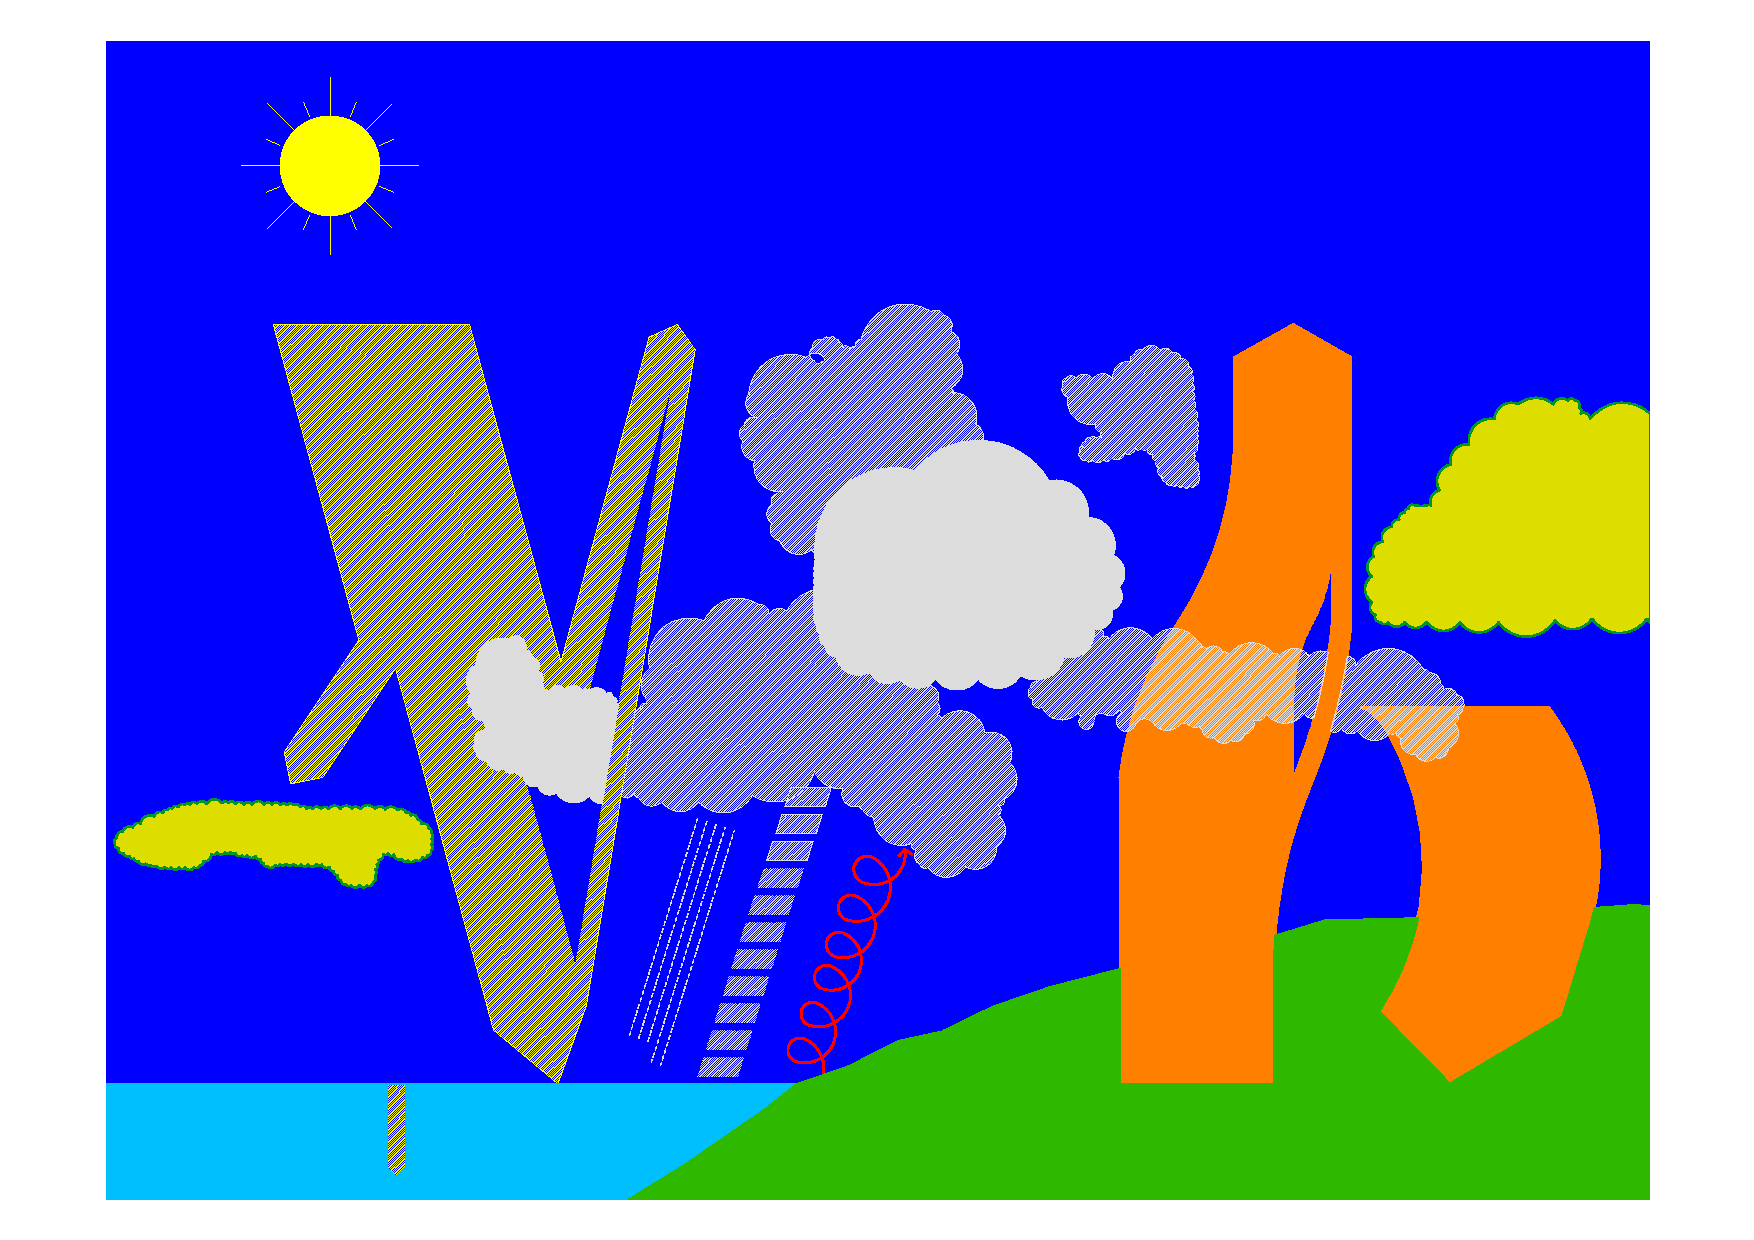
\includegraphics[scale = 0.55]{Chapter2_Theory/images/cre_ny_farge.pdf}};
        \begin{scope}
            % Grid to help find the positions (remove in final version)
            \node at (11cm, 19.5cm) {\Large \textcolor{mygray}{Cloud Radiative Effect (CRE)}};
            
            \node at (14.2cm, 18.1cm) {\Large \textcolor{orange}{LW CRE = +28}};
            %\node at (14.7cm, 16cm) {\large 28};
            
            \node at (9cm, 18.1cm) {\Large \textcolor{yellow}{SW CRE = -47}};
            %\node at (8.7cm, 16cm) {\large -47};
            
            
            % Litt usikker på om jeg syns de bidro
            %\node at (16.5cm, 15.4cm) {\large Atmosphere};
            %\node at (17cm, 18cm) {\large TOA};
            %\node at (16.4cm, 10.2cm) {\large Surface};
            
            \node [rotate = 70] at (10.5cm, 11.6cm) {\small \textcolor{red}{sensible heat}};
            \node [rotate = 73] at (9.7cm, 11.7cm) {\small \textcolor{mygray}{latent heat}};
            \node [rotate = 73] at (8.9cm, 11.5cm) {\small \textcolor{mygray}{solar reflected surface}};
            
            \node at (6.1cm, 10.7cm) {\small Imbalance};
            
            \node at (15.9cm, 11.2cm) {\Large 28};
            \node at (15.4cm, 14.1cm) {\Large 0};
            \node at (7.cm, 14.2cm) {\Large 7};
            \node at (11.2cm, 13.2cm) {\Large 7};
            
            \node at (11.3cm, 15.4cm) {\Large NET CRE};
            \node at (11.3cm, 14.9cm) {\Large =-19};
            
            \node at (11.cm, 10.6cm) {\Large -26};
             
            \node at (16.cm, 10.4cm) {\small thermal};
            \node at (16.cm, 10.1cm) {\small down};
            \node at (16.cm, 9.8cm) {\small surface};
            
            \node at (13.5cm, 11.4cm) {\small thermal};
            \node at (13.5cm, 11.1cm) {\small up};
            \node at (13.5cm, 10.9cm) {\small surface};
            
            \node at (7.6cm, 10.4cm) {\small solar}; % down surface
            \node at (7.6cm, 10.1cm) {\small down};
            \node at (7.6cm, 9.8cm) {\small surface};
            \node at (7.3cm, 11.3cm) {\textcolor{black}{\large -54}};
            
            \node at (5.9cm, 17.4cm) {\small incomming};
            \node at (5.9cm, 17.2cm) {\small solar};
            \node at (5.9cm, 16.90cm) {\small TOA};
            
            \node [rotate = 75] at (8.1cm, 16.cm) {\small solar reflected TOA};
            
            \node at (14.4cm, 17cm)   {\small thermal};
            \node at (14.4cm, 16.7cm) {\small outgoing};
            \node at (14.4cm, 16.4cm) {\small TOA};
            
            \node at (4.7cm, 13cm) {\small \textcolor{black}{solar absorbed}}; % atmosphere
            %\node at (4.38cm, 13.5cm) {\small \textcolor{black}{absored}}; % atmosphere
            \node at (4.6cm, 12.7cm) {\small \textcolor{black}{atmosphere}}; % atmosphere
        \end{scope}

    \end{tikzpicture}
    \caption{The global mean annual \acrfull{cre} is the difference between the radiative components of the clear-sky (cloud-free) and all-sky (cloudy) radiative components. A positive sign can be describes a warming effect and negative a cooling, units in $W m^{-2}$. Inspired by Figure 15 in \citepaper{Wild2019TheModels}.}
    \label{fig:cre}
\end{figure}
%%%%%%%%%%%%%%%%%%%%%%%%%%%%% WILD FIGURE 
%\begin{figure}[h]
%    \centering
%    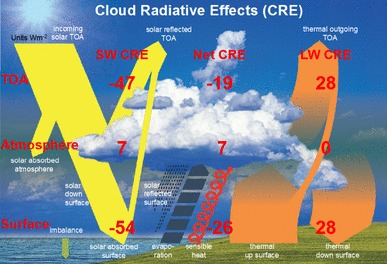
\includegraphics[scale = 7]{Chapter1_Intro/images/CRE_wild2019.jpg}
%    \caption{The global mean annual \acrfull{cre} is the difference between the radiative components of the clear-sky and all-sky radiative components. A positive sign can be described as a warming effect and negative a cooling, units in $W m^{-2}$. This schematic is a modified version of Figure 15 in \cite{Wild2019TheModels}.
%    }
%    \label{fig:cre}
%\end{figure}

Figure \ref{fig:cre} shows a schematic illustration of the \acrshort{cre} in the Earths TOA annual mean energy budget, a negative sign denotes a cooling effect and a positive sign can be associated with a warming effect. %, units are in $W m^{-2}$ 
\citepaper{Wild2019TheModels} find a reduction in incoming solar radiation of $-47Wm^{-2}$ caused by clouds, showing that clouds reflect approximately 50\% of the incoming solar radiation. The thermal \arcshort{cre} amounts to $28Wm^{-2}$, resulting in a net \acrshort{cre} of $-19Wm^{-2}$. This proves that the net effect of clouds on the TOA radiative budget is negative, and that clouds currently have a cooling effect on the climate. For the details on the all-sky (cloudy) and clear-sky (cloud-free) energy budgets, used in the computations of the \acrshort{cre}, please see the paper \citepaper{Wild2019TheModels}. %\textit{The cloud-free global energy balance and inferred cloud radiative effects: an assessment based on direct observations and climate models} by \cite{Wild2019TheModels}.

%Dense low level clouds reduce the amount of solar radiation absorbed by the surface, and the altitude of the clouds determine the amount of heat trapped in the system. 

\section{Clouds in future climates} \label{sec:intro_cloud_future_climates}
\begin{figure}[h]
    \centering
    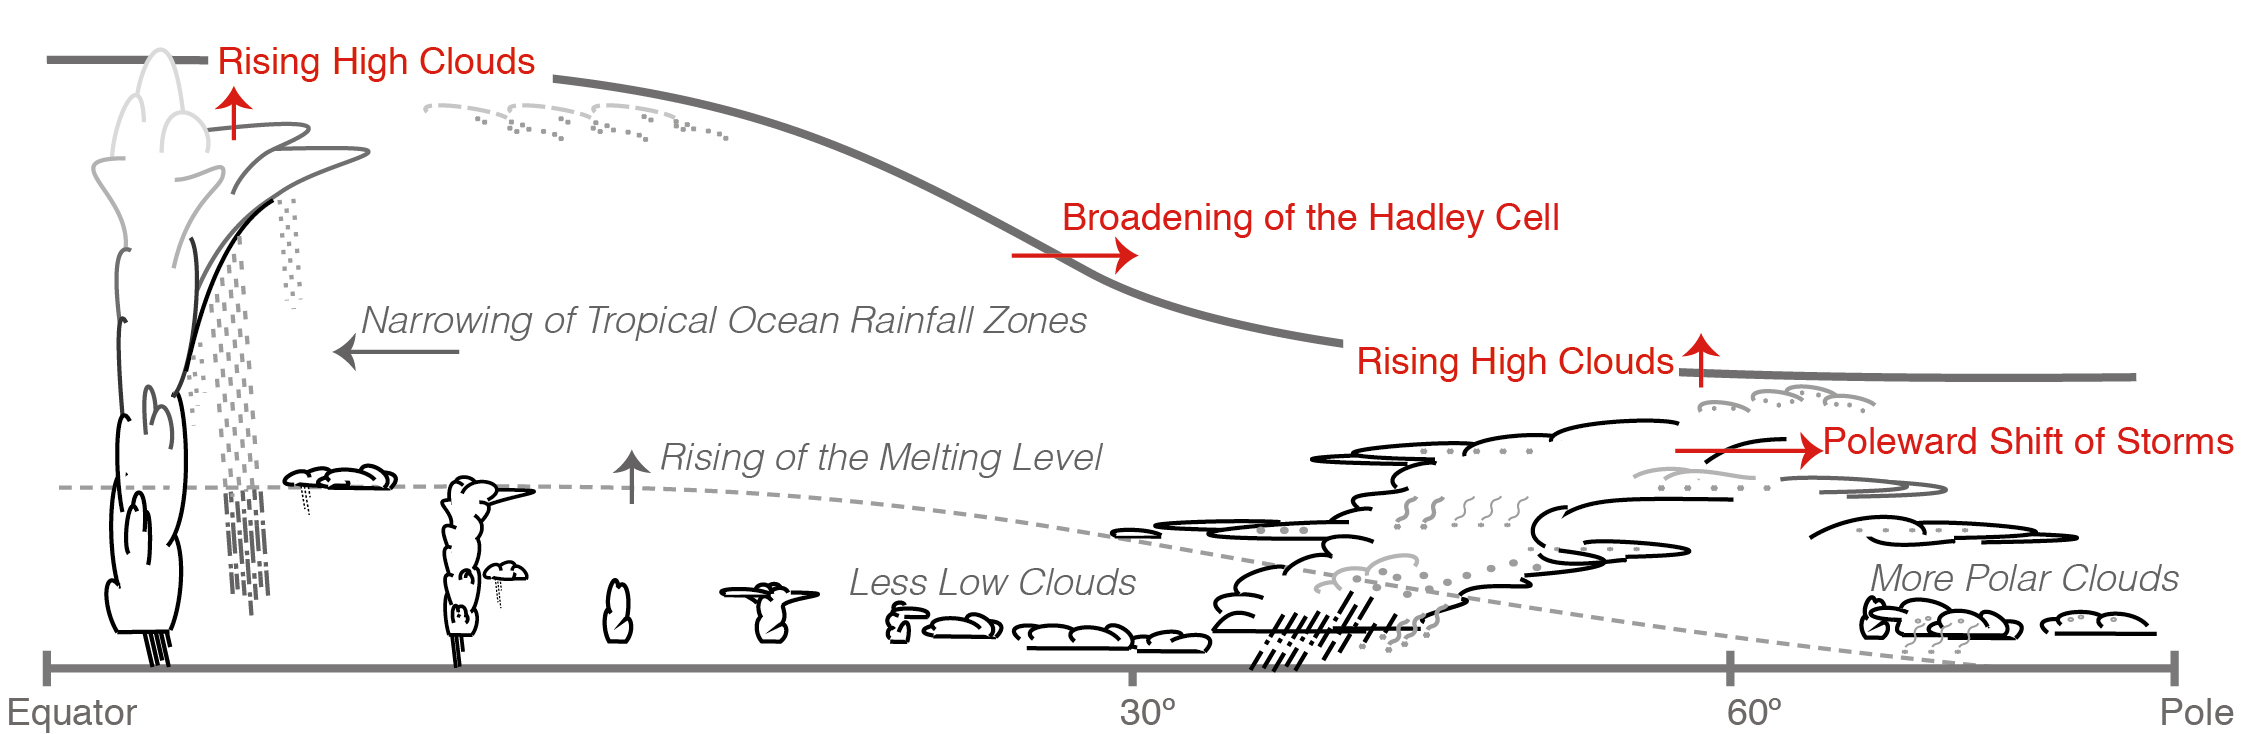
\includegraphics[scale = 0.8]{Chapter1_Intro/images/Fig7-11_ipcc.jpg}
    \caption{Expected cloud changes in future climate. This figure was developed based on feedbacks in climate models, and the different adjustments are associated with different levels of confidence.  (\cite{IPCC_CH7_clouds}).}
    \label{fig:cloud_scheme}
\end{figure}
As concluded in the previous section, an excess of radiation currently gets trapped in the Earth system, forcing the atmospheric temperature to increase in order to ultimately close the radiative budget. The temperature increase induces climate change and recent estimates find the imbalance at \acrshort{toa} to be $0.6 Wm^{-2}$ (\cite{Wild2019TheModels}).

Wild et. al. 2019  \textbf{siter} finds an imbalance of This heat gets trapped in the earth system, forcing the surface temperature to increase in order to close the radiative budget. 
The imbalance in the radiative budget at \acrfull{toa} is the radiative forcing. 
%TS: Hvorfor er teksten ovenfor kommentert ut? Den trengs jo for å definere "forcing"..
Climate drivers include both natural and anthropogenic forcings. A \textit{forcing} can be everything from natural variability in the solar energy output, volcanic eruptions or greenhouse gas emissions. The climate science community works toward a common goal to determine the magnitude of the forcings responsible for the observed climate change since pre-industrial times, and the associated climate response as quantified by the \arcshort{ecs}. The latter is controlled by climate feedback processes, of which those associated with clouds are the most uncertain. %Different emission scenarios result different \acrshort{ecs}.  

Figure \ref{fig:cloud_scheme} shows a summary of the most likely cloud feedbacks and the shift in cloud regimes suggested by the \acrshort{ipcc} (\cite{IPCC_CH7_clouds}).

First, a broadening of the Hadley cell causes a poleward shift of storms. This dries the subtropics and moistens the higher latitudes. Northward propagating clouds cause a reduction in the albedo effect. The radiation available for reflection decreases poleward, disappearing into the polar night, as a direct consequence of the Earth's spherical geometry.
%, caused by the spherical geometry of the Earth, the solar radiation available for reflection decrease poleward, until it disappears into the polar night \textcolor{red}{Altfor lang setning. Kanskje: "Northward propagating clouds would explain a reduction in the albedo effect
%. This is because/(as a concequence of)  the spherical geometry of the Earth decrease the solar radiation available for reflection poleward. Leading to a heating in the Arctics/at the poles as a consequence of/as as result of the greenhouse effect of clouds still persist without sunlight." Vet ikke om dette ble noe bedre, men jeg kan prøve å tenke litt videre på den. Den burde det uansett gjøres noe med :)}. 
%proportional with the $sin\left(\theta \right)$, where $\theta$ describes the latitude. 
The greenhouse effect of clouds still persist without sunlight leading to a heating due to clouds in the Arctic, in contrast to their global effect.
%TS: ta med en referanse her
Second, rising high clouds motivate a stronger greenhouse effect. Third, a reduction in the presence of low level clouds reduces the amount of reflected solar radiation.The reduced reflection of solar radiaton is assumed to be partly offset by an lifting of the melting layer. Consequently, ice crystals are replaced by liquid droplets and the phase transition results in more opaque clouds. 
%TS: legg til en referanse eller to her



\textit{Global radiative equilibrium} is reached when the temperature of the atmosphere is adjusted such that the radiation emitted to space is equal to the portion absorbed by the surface.
